\subsubsection{Flexion Image}\label{flexion-image-section}

The local shape of an object that is sampled by a depth sensor is characterized by its surface normal.
A surface normal is a vector perpendicular to the surface of the object.
The core idea of the \Gls{flexion-image} is the approximation of the surface normal with two different sets of neighbouring pixels and measuring their difference.

Each measured pixel is backprojected to camera coordinates, scaling the spherical coordinates with its measured range as first step.
The normal for a measured surface point $\mathbf{P_{i,j}}$ is calculated with the cross product of vectors connecting the neighbouring points of $\mathbf{P_{i,j}}$ (Equation~\ref{eq:flexion_normals}).
This point relationship is visualized in Figure~\ref{fig:flexion_normals_plane}.
\begin{figure}[ht]
    \begin{subfigure}[t]{0.48\linewidth}
        \centering
        \scalebox{1.0}{%
        

\tikzset{every picture/.style={line width=0.75pt}} %set default line width to 0.75pt        

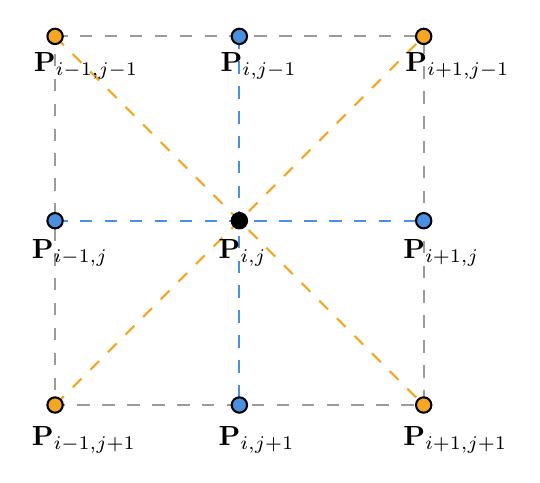
\begin{tikzpicture}[x=0.75pt,y=0.75pt,yscale=-1,xscale=1]
%uncomment if require: \path (0,237); %set diagram left start at 0, and has height of 237

%Shape: Rectangle [id:dp6565487036659107] 
\draw  [color={rgb, 255:red, 155; green, 155; blue, 155 }  ,draw opacity=1 ][dash pattern={on 4.5pt off 4.5pt}] (28.7,13.7) -- (206.3,13.7) -- (206.3,191.3) -- (28.7,191.3) -- cycle ;
%Straight Lines [id:da30195081571029425] 
\draw [color={rgb, 255:red, 74; green, 144; blue, 226 }  ,draw opacity=1 ] [dash pattern={on 4.5pt off 4.5pt}]  (28.7,102.5) -- (206.3,102.5) ;
%Straight Lines [id:da4586174781414081] 
\draw [color={rgb, 255:red, 74; green, 144; blue, 226 }  ,draw opacity=1 ] [dash pattern={on 4.5pt off 4.5pt}]  (117.5,13.7) -- (117.5,191.3) ;
%Straight Lines [id:da7294828306266232] 
\draw [color={rgb, 255:red, 245; green, 166; blue, 35 }  ,draw opacity=1 ] [dash pattern={on 4.5pt off 4.5pt}]  (28.7,13.7) -- (206.3,191.3) ;
%Straight Lines [id:da3243995266948473] 
\draw [color={rgb, 255:red, 245; green, 166; blue, 35 }  ,draw opacity=1 ] [dash pattern={on 4.5pt off 4.5pt}]  (28.7,191.3) -- (206.3,13.7) ;
%Shape: Circle [id:dp5266363779447065] 
\draw  [fill={rgb, 255:red, 245; green, 166; blue, 35 }  ,fill opacity=1 ] (25,13.7) .. controls (25,11.66) and (26.66,10) .. (28.7,10) .. controls (30.74,10) and (32.4,11.66) .. (32.4,13.7) .. controls (32.4,15.74) and (30.74,17.4) .. (28.7,17.4) .. controls (26.66,17.4) and (25,15.74) .. (25,13.7) -- cycle ;
%Shape: Ellipse [id:dp14497174740803043] 
\draw  [fill={rgb, 255:red, 74; green, 144; blue, 226 }  ,fill opacity=1 ] (25,102.5) .. controls (25,100.46) and (26.66,98.8) .. (28.7,98.8) .. controls (30.74,98.8) and (32.4,100.46) .. (32.4,102.5) .. controls (32.4,104.54) and (30.74,106.2) .. (28.7,106.2) .. controls (26.66,106.2) and (25,104.54) .. (25,102.5) -- cycle ;
%Shape: Ellipse [id:dp0427609892023727] 
\draw  [fill={rgb, 255:red, 245; green, 166; blue, 35 }  ,fill opacity=1 ] (25,191.3) .. controls (25,189.26) and (26.66,187.6) .. (28.7,187.6) .. controls (30.74,187.6) and (32.4,189.26) .. (32.4,191.3) .. controls (32.4,193.34) and (30.74,195) .. (28.7,195) .. controls (26.66,195) and (25,193.34) .. (25,191.3) -- cycle ;
%Shape: Ellipse [id:dp2872052196845898] 
\draw  [fill={rgb, 255:red, 74; green, 144; blue, 226 }  ,fill opacity=1 ] (113.8,13.7) .. controls (113.8,11.66) and (115.46,10) .. (117.5,10) .. controls (119.54,10) and (121.2,11.66) .. (121.2,13.7) .. controls (121.2,15.74) and (119.54,17.4) .. (117.5,17.4) .. controls (115.46,17.4) and (113.8,15.74) .. (113.8,13.7) -- cycle ;
%Shape: Circle [id:dp758793708555806] 
\draw  [fill={rgb, 255:red, 0; green, 0; blue, 0 }  ,fill opacity=1 ] (113.8,102.5) .. controls (113.8,100.46) and (115.46,98.8) .. (117.5,98.8) .. controls (119.54,98.8) and (121.2,100.46) .. (121.2,102.5) .. controls (121.2,104.54) and (119.54,106.2) .. (117.5,106.2) .. controls (115.46,106.2) and (113.8,104.54) .. (113.8,102.5) -- cycle ;
%Shape: Circle [id:dp477059334030714] 
\draw  [fill={rgb, 255:red, 74; green, 144; blue, 226 }  ,fill opacity=1 ] (113.8,191.3) .. controls (113.8,189.26) and (115.46,187.6) .. (117.5,187.6) .. controls (119.54,187.6) and (121.2,189.26) .. (121.2,191.3) .. controls (121.2,193.34) and (119.54,195) .. (117.5,195) .. controls (115.46,195) and (113.8,193.34) .. (113.8,191.3) -- cycle ;
%Shape: Ellipse [id:dp13207731000753575] 
\draw  [fill={rgb, 255:red, 245; green, 166; blue, 35 }  ,fill opacity=1 ] (202.6,13.7) .. controls (202.6,11.66) and (204.26,10) .. (206.3,10) .. controls (208.34,10) and (210,11.66) .. (210,13.7) .. controls (210,15.74) and (208.34,17.4) .. (206.3,17.4) .. controls (204.26,17.4) and (202.6,15.74) .. (202.6,13.7) -- cycle ;
%Shape: Circle [id:dp8288145253462365] 
\draw  [fill={rgb, 255:red, 74; green, 144; blue, 226 }  ,fill opacity=1 ] (202.6,102.5) .. controls (202.6,100.46) and (204.26,98.8) .. (206.3,98.8) .. controls (208.34,98.8) and (210,100.46) .. (210,102.5) .. controls (210,104.54) and (208.34,106.2) .. (206.3,106.2) .. controls (204.26,106.2) and (202.6,104.54) .. (202.6,102.5) -- cycle ;
%Shape: Circle [id:dp9160642610677009] 
\draw  [fill={rgb, 255:red, 245; green, 166; blue, 35 }  ,fill opacity=1 ] (202.6,191.3) .. controls (202.6,189.26) and (204.26,187.6) .. (206.3,187.6) .. controls (208.34,187.6) and (210,189.26) .. (210,191.3) .. controls (210,193.34) and (208.34,195) .. (206.3,195) .. controls (204.26,195) and (202.6,193.34) .. (202.6,191.3) -- cycle ;

% Text Node
\draw (106,110) node [anchor=north west][inner sep=0.75pt]   [align=left] {$\displaystyle \mathbf{P}_{i,j}$};
% Text Node
\draw (195,110) node [anchor=north west][inner sep=0.75pt]   [align=left] {$\displaystyle \mathbf{P}_{i+1,j}$};
% Text Node
\draw (16,110) node [anchor=north west][inner sep=0.75pt]   [align=left] {$\displaystyle \mathbf{P}_{i-1,j}$};
% Text Node
\draw (107,20) node [anchor=north west][inner sep=0.75pt]   [align=left] {$\displaystyle \mathbf{P}_{i,j-1}$};
% Text Node
\draw (196,20) node [anchor=north west][inner sep=0.75pt]   [align=left] {$\displaystyle \mathbf{P}_{i+1,j-1}$};
% Text Node
\draw (17,20) node [anchor=north west][inner sep=0.75pt]   [align=left] {$\displaystyle \mathbf{P}_{i-1,j-1}$};
% Text Node
\draw (106,200) node [anchor=north west][inner sep=0.75pt]   [align=left] {$\displaystyle \mathbf{P}_{i,j+1}$};
% Text Node
\draw (195,200) node [anchor=north west][inner sep=0.75pt]   [align=left] {$\displaystyle \mathbf{P}_{i+1,j+1}$};
% Text Node
\draw (16,200) node [anchor=north west][inner sep=0.75pt]   [align=left] {$\displaystyle \mathbf{P}_{i-1,j+1}$};


\end{tikzpicture}


        }
        \caption{The normals for a point $\mathbf{P_{i,j}}$ can be estimated by either its diagonal or horizontal and vertical neighbours.}\label{fig:flexion_normals_plane}
    \end{subfigure}\quad
    \begin{subfigure}[t]{0.49\linewidth}
        \centering
        \scalebox{1.0}{%
        \begin{tikzpicture}
    \node[anchor=south west,inner sep=0] (image) at (4.0,0) {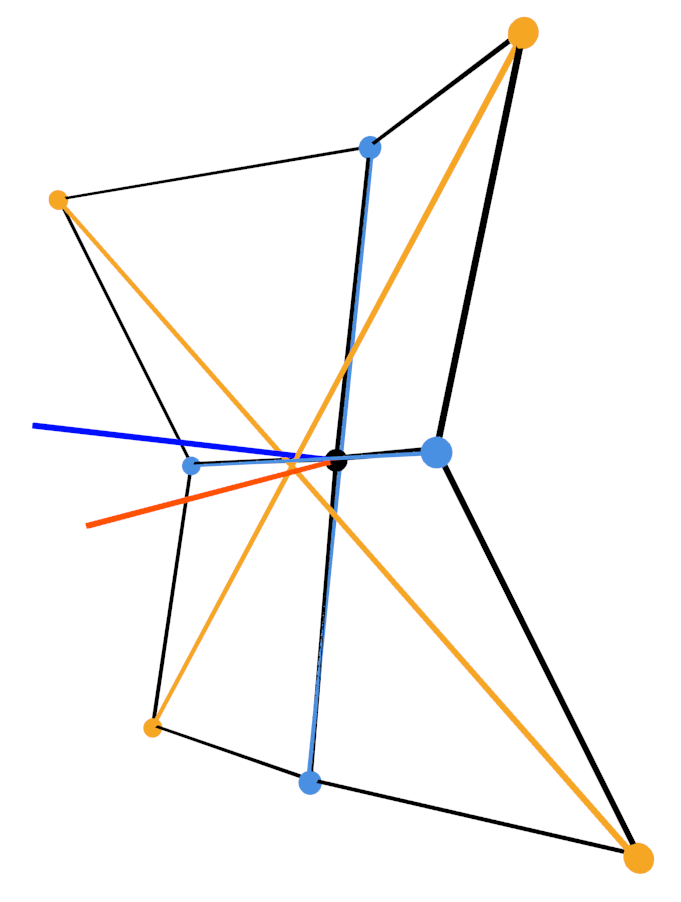
\includegraphics[width=0.6\textwidth]{chapter04/img/flexion-model-2-clipped.png}};
    \node at (4.4, 5.1) {$\mathbf{P_{i-1,j-1}}$};
    \node at (6.2, 5.5) {$\mathbf{P_{i,j-1}}$};
    \node at (8.5, 5.8) {$\mathbf{P_{i+1,j-1}}$};

    \node at (4.7, 2.9) {\scalebox{0.9}{$\mathbf{P_{i-1,j}}$}};
    \node at (6.2, 2.5) {$\mathbf{P_{i,j}}$};
    \node at (7.7, 3.0) {$\mathbf{P_{i+1,j}}$};

    \node at (5.0, 0.9) {$\mathbf{P_{i-1,j+1}}$};
    \node at (6.3, 0.4) {$\mathbf{P_{i,j+1}}$};
    \node at (9.2, 0.3) {$\mathbf{P_{i+1,j+1}}$};

    \node [plotdarkblue] at (4.6, 3.5) {$\vec{n_1}$};
    \node [plotdarkorange] at (4.8, 2.3) {$\vec{n_2}$};
\end{tikzpicture}

        }
        \caption{The estimated normals span an angle depending on the local shape of the measured surface.}\label{fig:flexion_space}
    \end{subfigure}
    \caption[Schematic representation of the \gls{flexion-image} calculation]{\emph{Schematic representation of the \gls{flexion-image} calculation.} This figure demonstrates how non-planar surfaces have different normals for diagonal and non-diagonal estimation. This difference is utilized as measure for flexion.}%
    \label{fig:flexion-image-scetched}
\end{figure}
Using the diagonal and vertical neighbouring points (blue) results in a different normal than the diagonal neighbours (orange) do.
As Figure~\ref{fig:flexion_space} demonstrates, both normals span an angle.

\begin{equation}
\begin{aligned}
    \vec{n_1} &= \frac{\vec{P_{i,j-1}} - \vec{P_{i,j+1}}}{\lnorm{\vec{P_{i,j-1}} - \vec{P_{i,j+1}}}}
                \times \frac{\vec{P_{i-1,j}} - \vec{P_{i+1,j}}}{\lnorm{\vec{P_{i-1,j}} - \vec{P_{i+1,j}}}} \\
    \vec{n_2} &= \frac{\vec{P_{i-1,j-1}} - \vec{P_{i+1,j+1}}}{\lnorm{\vec{P_{i-1,j-1}} - \vec{P_{i+1,j+1}}}}
                \times \frac{\vec{P_{i-1,j+1}} - \vec{P_{i+1,j-1}}}{\lnorm{\vec{P_{i-1,j+1}} - \vec{P_{i+1,j-1}}}}
    \label{eq:flexion_normals}
\end{aligned}
\end{equation}
It shall be pointed out, that both normals $\vec{n_1}$ and $\vec{n_2}$ are not unit length.
Finally, the Flexion $\mathcal{F}$ of point $\mathbf{P_{i,j}}$ is defined as:
\begin{align}
    \mathcal{F} &= \abs{\vec{n_1} \cdotp \vec{n_2}}\text{.}
\end{align}
Because $\lnorm{\vec{n_1}},\lnorm{\vec{n_2}} \in [0,1]$ the value of is bound to $\mathcal{F} \in [0, 1]$.
Creating the final image requires a linear scaling to the desired output image depth using Equation~\ref{eq:linear_scaling}.

\subsubsection*{Characteristics}

\begin{figure}[tb]
    \begin{subfigure}[t]{0.32\textwidth}
        
\includegraphics[width=\linewidth]{chapter04/img/flexion-0001.png}
    \end{subfigure}
    \begin{subfigure}[t]{0.32\textwidth}
        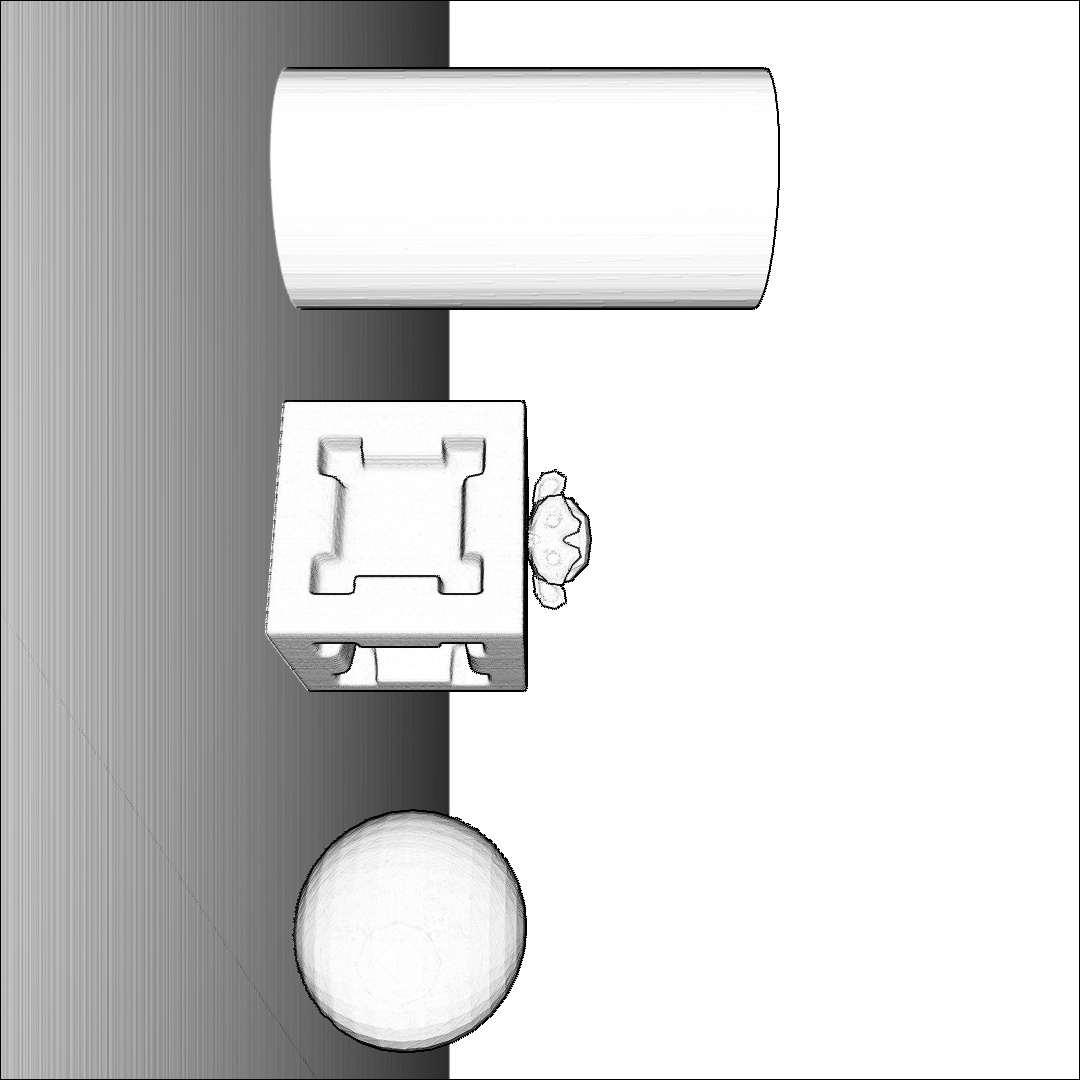
\includegraphics[width=\linewidth]{chapter04/img/flexion-0030.png}
    \end{subfigure}
    \begin{subfigure}[t]{0.32\textwidth}
        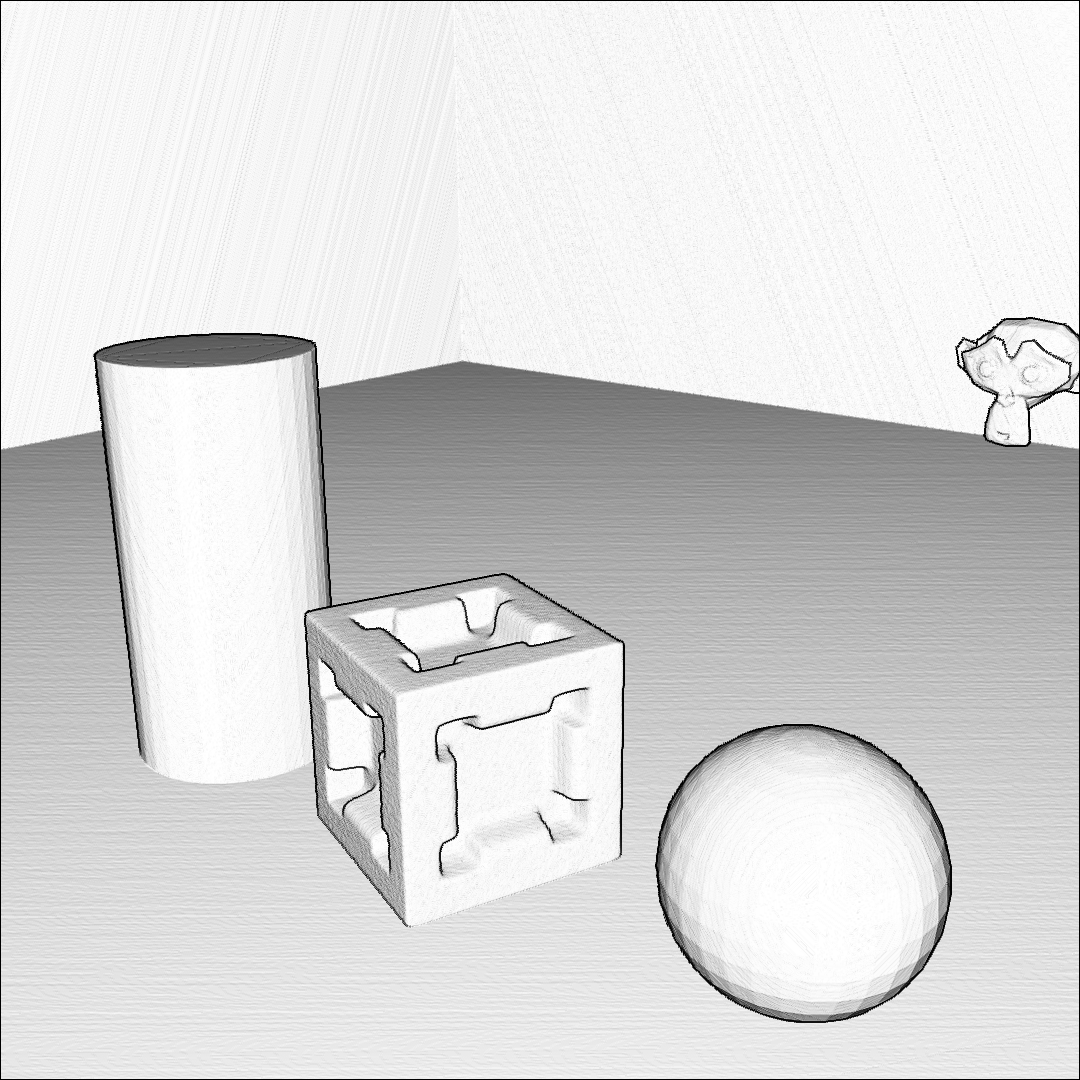
\includegraphics[width=\linewidth]{chapter04/img/flexion-0210.png}
    \end{subfigure}
    \caption[Characterstic look of a \gls{flexion-image}]{\emph{Characterstic look of a \gls{flexion-image}.} These figures demonstrate the characteristic look of \Glspl{flexion-image}. Their appearence is very plastic and the shading effects give a good sense for depth. The conversion is rotation invariant.}\label{fig:flexion_images}
\end{figure}
Figure~\ref{fig:flexion_images} visualizes the \Gls{flexion-image} for the same camera positions as for the other feature images.
The \gls{flexion-image} is rotation invariant.
Rotation of either an object or the camera does not change the difference between the two normal approximations.
A flat surface has an almost constant shading, because the normal approximation results in the same vector directions.
Flat surfaces not perpendicular to the camera plane have non-constant shading with the brightness reducing the further the surface patch is appart from the camera center.
This effect is caused by the perspective transformation.
The norm of cross product is maximal if both multiplied vectors are perpendicular:
\begin{equation}
    \lnorm{\vec{v_1} \times \vec{v_2}} = \lnorm{\vec{v_1}} \lnorm{\vec{v_2}} \sin \angle(\vec{v_1}, \vec{v_2})\text{.}
\end{equation}
Because the vectors multiplied to form the normals $n_1$ and $n_2$ have different angles based on their distance to the camera (Figure~\ref{fig:flexion_angle_decrease}), the lengths of the normals differ throughout the image.
The lack of normalization in Equation~\ref{eq:flexion_normals} propagates this effect through to the scalar product, as the length of the both vectors are multiplied:
\begin{equation}
    \vec{v_1} \cdot \vec{v_2} = \lnorm{\vec{v_1}} \lnorm{\vec{v_2}} \cos \angle(\vec{v_1}, \vec{v_2})\text{.}
\end{equation}
\begin{figure}[b!]
    

\tikzset{every picture/.style={line width=0.75pt}} %set default line width to 0.75pt        

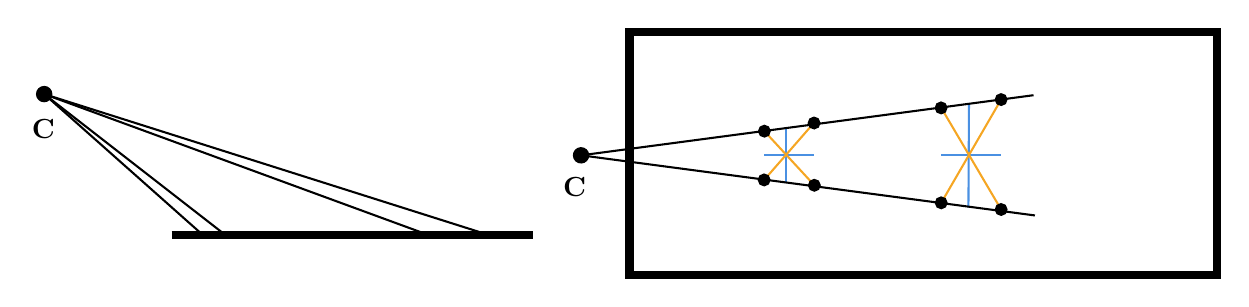
\begin{tikzpicture}[x=0.75pt,y=0.75pt,yscale=-1,xscale=1]
%uncomment if require: \path (0,142); %set diagram left start at 0, and has height of 142

%Straight Lines [id:da6840514143989631] 
\draw [color={rgb, 255:red, 74; green, 144; blue, 226 }  ,draw opacity=1 ]   (366.4,69.04) -- (390.44,69.04) ;
%Straight Lines [id:da9689027017272559] 
\draw [color={rgb, 255:red, 74; green, 144; blue, 226 }  ,draw opacity=1 ]   (377.02,82.13) -- (377.02,55.88) ;
%Straight Lines [id:da8683032061954556] 
\draw [color={rgb, 255:red, 74; green, 144; blue, 226 }  ,draw opacity=1 ]   (451.65,69.04) -- (480.52,69.04) ;
%Straight Lines [id:da6934594327602702] 
\draw [color={rgb, 255:red, 74; green, 144; blue, 226 }  ,draw opacity=1 ]   (464.75,94.04) -- (465.02,44.04) ;
%Straight Lines [id:da7261021710957941] 
\draw [color={rgb, 255:red, 245; green, 166; blue, 35 }  ,draw opacity=1 ]   (480.5,42.14) -- (451.64,91.89) ;
%Straight Lines [id:da37992799055918147] 
\draw [color={rgb, 255:red, 245; green, 166; blue, 35 }  ,draw opacity=1 ]   (451.58,46) -- (480.5,95.1) ;
%Straight Lines [id:da15457235634391941] 
\draw [color={rgb, 255:red, 245; green, 166; blue, 35 }  ,draw opacity=1 ]   (389.38,54.43) -- (366.33,80.86) ;
%Straight Lines [id:da05878950535382432] 
\draw [color={rgb, 255:red, 245; green, 166; blue, 35 }  ,draw opacity=1 ]   (366.45,57.36) -- (390.5,83.43) ;
%Straight Lines [id:da045550454885305736] 
\draw [line width=3]    (80.9,107.5) -- (254.9,107.5) ;
%Shape: Circle [id:dp8549507101465224] 
\draw  [fill={rgb, 255:red, 0; green, 0; blue, 0 }  ,fill opacity=1 ] (16,39.5) .. controls (16,37.59) and (17.54,36.05) .. (19.45,36.05) .. controls (21.36,36.05) and (22.9,37.59) .. (22.9,39.5) .. controls (22.9,41.41) and (21.36,42.95) .. (19.45,42.95) .. controls (17.54,42.95) and (16,41.41) .. (16,39.5) -- cycle ;
%Straight Lines [id:da09684243305909856] 
\draw    (19.45,39.5) -- (94.9,106.5) ;
%Straight Lines [id:da4476141598512392] 
\draw    (19.45,39.5) -- (106.9,107.5) ;
%Straight Lines [id:da5555101325179832] 
\draw    (19.45,39.5) -- (204.9,107.5) ;
%Straight Lines [id:da06573307117836547] 
\draw    (19.45,39.5) -- (230.9,106.5) ;
%Shape: Circle [id:dp3195203497272404] 
\draw  [fill={rgb, 255:red, 0; green, 0; blue, 0 }  ,fill opacity=1 ] (274.67,69.08) .. controls (274.62,67.18) and (276.13,65.6) .. (278.04,65.55) .. controls (279.94,65.51) and (281.52,67.02) .. (281.57,68.92) .. controls (281.61,70.83) and (280.1,72.41) .. (278.2,72.45) .. controls (276.29,72.49) and (274.71,70.99) .. (274.67,69.08) -- cycle ;
%Straight Lines [id:da25083036265050096] 
\draw    (278.12,69) -- (496.79,97.97) ;
%Straight Lines [id:da6083860800665152] 
\draw    (278.12,69) -- (496.1,40.04) ;
%Shape: Rectangle [id:dp031034421219254926] 
\draw  [line width=3]  (301.4,9.5) -- (584.4,9.5) -- (584.4,126.5) -- (301.4,126.5) -- cycle ;
%Shape: Circle [id:dp2988386895287467] 
\draw  [fill={rgb, 255:red, 0; green, 0; blue, 0 }  ,fill opacity=1 ] (363.85,57.42) .. controls (363.81,55.99) and (364.95,54.8) .. (366.39,54.76) .. controls (367.82,54.73) and (369.01,55.87) .. (369.05,57.3) .. controls (369.08,58.74) and (367.94,59.93) .. (366.51,59.96) .. controls (365.07,60) and (363.88,58.86) .. (363.85,57.42) -- cycle ;
%Shape: Circle [id:dp49087747494377276] 
\draw  [fill={rgb, 255:red, 0; green, 0; blue, 0 }  ,fill opacity=1 ] (363.73,80.92) .. controls (363.69,79.48) and (364.83,78.29) .. (366.27,78.26) .. controls (367.7,78.23) and (368.89,79.36) .. (368.93,80.8) .. controls (368.96,82.23) and (367.82,83.42) .. (366.39,83.46) .. controls (364.95,83.49) and (363.76,82.35) .. (363.73,80.92) -- cycle ;
%Shape: Circle [id:dp3291682457892863] 
\draw  [fill={rgb, 255:red, 0; green, 0; blue, 0 }  ,fill opacity=1 ] (387.79,53.49) .. controls (387.75,52.06) and (388.89,50.87) .. (390.32,50.84) .. controls (391.76,50.8) and (392.95,51.94) .. (392.98,53.37) .. controls (393.02,54.81) and (391.88,56) .. (390.44,56.03) .. controls (389.01,56.07) and (387.82,54.93) .. (387.79,53.49) -- cycle ;
%Shape: Circle [id:dp598750640317177] 
\draw  [fill={rgb, 255:red, 0; green, 0; blue, 0 }  ,fill opacity=1 ] (387.91,83.49) .. controls (387.87,82.05) and (389.01,80.86) .. (390.44,80.83) .. controls (391.88,80.79) and (393.07,81.93) .. (393.1,83.37) .. controls (393.14,84.8) and (392,85.99) .. (390.56,86.03) .. controls (389.13,86.06) and (387.94,84.92) .. (387.91,83.49) -- cycle ;
%Shape: Circle [id:dp3156912690396848] 
\draw  [fill={rgb, 255:red, 0; green, 0; blue, 0 }  ,fill opacity=1 ] (449.04,91.95) .. controls (449.01,90.51) and (450.14,89.32) .. (451.58,89.29) .. controls (453.02,89.26) and (454.21,90.39) .. (454.24,91.83) .. controls (454.27,93.26) and (453.13,94.45) .. (451.7,94.49) .. controls (450.26,94.52) and (449.07,93.38) .. (449.04,91.95) -- cycle ;
%Shape: Circle [id:dp0381257221295519] 
\draw  [fill={rgb, 255:red, 0; green, 0; blue, 0 }  ,fill opacity=1 ] (448.99,46.21) .. controls (448.95,44.77) and (450.09,43.58) .. (451.53,43.55) .. controls (452.96,43.52) and (454.15,44.65) .. (454.18,46.09) .. controls (454.22,47.53) and (453.08,48.72) .. (451.65,48.75) .. controls (450.21,48.78) and (449.02,47.65) .. (448.99,46.21) -- cycle ;
%Shape: Circle [id:dp4047969379608699] 
\draw  [fill={rgb, 255:red, 0; green, 0; blue, 0 }  ,fill opacity=1 ] (477.91,42.2) .. controls (477.87,40.76) and (479.01,39.57) .. (480.44,39.54) .. controls (481.88,39.51) and (483.07,40.64) .. (483.1,42.08) .. controls (483.14,43.51) and (482,44.7) .. (480.56,44.74) .. controls (479.13,44.77) and (477.94,43.63) .. (477.91,42.2) -- cycle ;
%Shape: Circle [id:dp5781527725767942] 
\draw  [fill={rgb, 255:red, 0; green, 0; blue, 0 }  ,fill opacity=1 ] (477.91,95.16) .. controls (477.87,93.72) and (479.01,92.53) .. (480.44,92.5) .. controls (481.88,92.46) and (483.07,93.6) .. (483.1,95.04) .. controls (483.14,96.47) and (482,97.66) .. (480.56,97.69) .. controls (479.13,97.73) and (477.94,96.59) .. (477.91,95.16) -- cycle ;

% Text Node
\draw (12,50.05) node [anchor=north west][inner sep=0.75pt]   [align=left] {$\displaystyle \mathbf{C}$};
% Text Node
\draw (268,78.05) node [anchor=north west][inner sep=0.75pt]   [align=left] {$\displaystyle \mathbf{C}$};


\end{tikzpicture}

    \caption[Explanation of shading effect in \glspl{flexion-image}]{\emph{Explanation of shading effect in \glspl{flexion-image}.} The angle between the diagonals decreases with increasing distance from the camera center. This results in shorter normals.}\label{fig:flexion_angle_decrease}
\end{figure}
